% 回収テストの節の下書き（2026-10-16）。結果が届いたら EML_supplementary.tex の sec:S_ident の後ろに \input する。
% 数字はすべて \TBD。表は tools/recovery_evaluate.py の <out>.tex をそのまま \input（手で直さない）。
% 評価の手順（CH）:
%   python3 tools/recovery_evaluate.py \
%     --case "CH=docs/revision/generated/recovery_runs/CH_syn_n1_r0/synthetic.json=docs/revision/generated/recovery_runs/CH_syn_n1_r0_2c_raw_seed*" \
%     --out docs/revision/EML_submission/figures/raw/recovery
% 10/16 にクラウドで模擬の入力（実 run を回復 run の代わり）で通ることを確認済み。合成データの log L(θ_true) = −20.946（72 パーセンタイル）。
\section{Recovery test on synthetic data}
\label{sec:S_recovery}
To test whether the pipeline recovers known interaction coefficients, and whether the classification of Section~\ref{sec:S_ident} reflects the information in the data rather than the sampler, we generated synthetic data from a point of the CH posterior (the best particle of the stage-(iv) seed with the highest log-likelihood at the time, $-26.52$) at the measured time points, with Gaussian noise of the same standard deviations as in the likelihood (viable and total-count compositions and live fraction), and inferred them again with the stage-(iv) settings (box, weights, 5000 particles, 150 mutation steps) and three seeds.
The log-likelihood of the true parameters on the synthetic data, $-20.95$, lies at the 72nd percentile of its distribution over noise realisations, so the realisation is typical; the three seeds reach $-18.98$ to $-19.03$ and meet criteria (a)--(e) (11 moves per free parameter, spread of the maximum log-likelihood 0.05, of the medians 0.05 posterior SD).
The classification is reproduced entry by entry (Table~\ref{tab:S_recovery}, Fig.~\ref{fig:S_recovery}): the six entries identified on the measured data are identified again on the synthetic data, and the nine entries not identified on the measured data are not identified on the synthetic data either, although their true values are known and, for four of them, lie close to a bound of the box.
Entries reported as not identified are therefore not identified even when the model is correct: this is a property of the data, not of the sampler.
The point recovery of the identified entries is weaker: only two of the six 90\% intervals contain the true value, and the posterior medians differ from the truth by up to 0.34 of the box width ($a_{22}$: truth $+0.50$, posterior $-0.35$ $[-0.92,+0.40]$; $a_{33}$: $-0.71$ against $-4.5$ $[-7.6,-1.5]$), while the sampler finds parameters that fit the noisy data better than the truth ($-19.0$ against $-20.95$).
Over all 15 entries, 8 intervals contain the true value.
Because the truth is a single point, the coverage of the 90\% intervals is not an independent 0.9 trial per entry (entries are correlated, and Bayesian coverage is an average over the prior); but the under-coverage of the identified entries is consistent with the likelihood treating the species fractions as independent (main text, Section~4.5), and the posterior intervals of the identified entries should be read as lower bounds on their uncertainty.
The same test on CS and DS (synthetic data from the best particle of the final-stage seed with the highest log-likelihood; 15000 and 54000 particles; criteria (a)--(e) met) gives the same picture with better point recovery: in CS all five identified entries are identified again and contain the true value (largest error 0.21 of the box width), and the nine not identified remain so; the one change of class is $a_{12}$, sign-only on the measured data and not identified on the synthetic data (its true value, $+1.35$, is recovered: median $+1.24$ $[-0.07,+1.93]$). In DS, eight of the nine identified entries are identified again and contain the true value (largest error 0.21), $a_{13}$ becomes sign-only with the true value inside its interval, $a_{25}$ (true $+2.49$ near the upper bound of the box) is identified but its interval $[+0.84,+2.46]$ just misses the truth, and the six not identified remain so; coverage over all 15 entries is 13/15 in both conditions. In DH (synthetic data from the best particle of the stage-(iii) seed with the highest log-likelihood; 60000 particles; criteria met) all eight identified entries are identified again with the true value inside the interval (largest error 0.13 of the box width), the seven not identified remain so, and all 15 intervals contain the truth; this realisation is, however, a favourable one (the log-likelihood of the true parameters, $-18.75$, lies at the 97th percentile of its distribution over noise realisations, against the 60th--72nd percentile in the other conditions).

\begin{figure}[h]
\centering
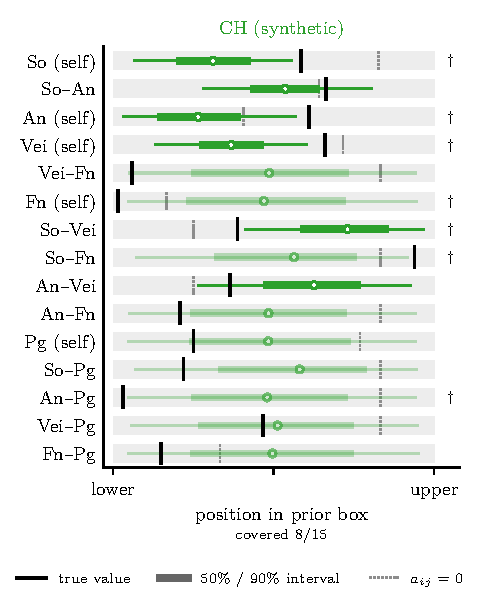
\includegraphics[width=\textwidth]{figures/raw/recovery.pdf}
\caption{Recovery test: posterior on the synthetic data (thick bar 50\%, thin bar 90\% interval, circle median) and true value (black tick), drawn as position within the prior box of each entry; pale: not identified. $\dagger$: interval does not contain the true value. Generated by \texttt{tools/recovery\_evaluate.py}.}
\label{fig:S_recovery}
\end{figure}

\begin{table}[h]
\centering
\caption{Recovery test (four conditions): true value, posterior median and 90\% interval on the synthetic data, ratio of the posterior SD to that of a uniform distribution on the box, and classification on the synthetic and on the measured data (id., identified; n.i., not identified). $^\dagger$: interval does not contain the true value. Generated by \texttt{tools/recovery\_evaluate.py}.}
\label{tab:S_recovery}
\footnotesize
\IfFileExists{figures/raw/recovery.tex}{% tools/recovery_evaluate.py が生成（手で直さない）。列: 真値、合成データでの事後中央値 [5%, 95%]（真値を含まなければ太字＋†）、分類（合成 / 実データ、違えば斜体）。2 条件ずつの段
\begin{tabular}{@{}lrlcrlc@{}}
\toprule
Entry & \multicolumn{3}{c}{CH} & \multicolumn{3}{c}{CS}\\
 & truth & median [5\%, 95\%] & synth./real & truth & median [5\%, 95\%] & synth./real\\
\midrule
$a_{11}$ & $-0.58$ & \textbf{$-1.25$ [$-1.85$, $-0.66$]}$^{\dagger}$ & id./id. & $-4.02$ & $-4.34$ [$-7.80$, $-1.45$] & id./id.\\
$a_{12}$ & $+0.05$ & $-0.23$ [$-0.79$, $+0.36$] & id./id. & $+1.35$ & $+1.24$ [$-0.07$, $+1.93$] & \textit{n.i./s.o.}\\
$a_{22}$ & $+0.50$ & \textbf{$-0.35$ [$-0.92$, $+0.40$]}$^{\dagger}$ & id./id. & $+1.60$ & $+0.79$ [$-0.31$, $+1.80$] & id./id.\\
$a_{33}$ & $-0.71$ & \textbf{$-4.52$ [$-7.59$, $-1.48$]}$^{\dagger}$ & id./id. & $-11.24$ & $-9.78$ [$-14.50$, $-3.42$] & id./id.\\
$a_{34}$ & $-4.65$ & $-2.08$ [$-4.70$, $+0.65$] & n.i./n.i. & $+0.85$ & \textbf{$-2.00$ [$-4.70$, $+0.68$]}$^{\dagger}$ & n.i./n.i.\\
$a_{44}$ & $-0.91$ & \textbf{$+1.82$ [$-0.72$, $+4.66$]}$^{\dagger}$ & n.i./n.i. & $+0.15$ & $-0.00$ [$-0.90$, $+0.90$] & n.i./n.i.\\
$a_{13}$ & $+0.55$ & \textbf{$+1.92$ [$+0.65$, $+2.87$]}$^{\dagger}$ & id./id. & $+8.28$ & $+7.75$ [$+3.34$, $+11.35$] & id./id.\\
$a_{14}$ & $+0.63$ & \textbf{$-1.62$ [$-4.56$, $+0.51$]}$^{\dagger}$ & n.i./n.i. & $-0.02$ & $-1.85$ [$-4.69$, $+0.70$] & n.i./n.i.\\
$a_{23}$ & $+0.46$ & $+1.50$ [$+0.07$, $+2.71$] & id./id. & $-0.39$ & $-0.22$ [$-1.34$, $+1.52$] & id./id.\\
$a_{24}$ & $-3.74$ & $-2.09$ [$-4.68$, $+0.65$] & n.i./n.i. & $-3.92$ & $-2.01$ [$-4.71$, $+0.71$] & n.i./n.i.\\
$a_{55}$ & $-3.37$ & $-1.86$ [$-4.69$, $+1.13$] & n.i./n.i. & $-0.44$ & $-0.00$ [$-0.90$, $+0.90$] & n.i./n.i.\\
$a_{15}$ & $-3.68$ & $-1.51$ [$-4.58$, $+0.68$] & n.i./n.i. & $-2.20$ & $-1.78$ [$-4.67$, $+0.71$] & n.i./n.i.\\
$a_{25}$ & $-4.81$ & \textbf{$-2.12$ [$-4.71$, $+0.65$]}$^{\dagger}$ & n.i./n.i. & $-1.62$ & $-1.89$ [$-4.69$, $+0.72$] & n.i./n.i.\\
$a_{35}$ & $-2.19$ & $-1.92$ [$-4.66$, $+0.70$] & n.i./n.i. & $-0.83$ & $-1.93$ [$-4.70$, $+0.70$] & n.i./n.i.\\
$a_{45}$ & $-0.55$ & $+0.49$ [$-0.85$, $+1.86$] & n.i./n.i. & $+0.92$ & \textbf{$-0.00$ [$-0.90$, $+0.89$]}$^{\dagger}$ & n.i./n.i.\\
\midrule
\multicolumn{1}{@{}l}{} & \multicolumn{3}{l}{covered 8/15 (identified 2/6); re-identified 6/6} & \multicolumn{3}{l}{covered 13/15 (identified 5/5); re-identified 5/5}\\
\bottomrule
\end{tabular}
\par\medskip
\begin{tabular}{@{}lrlcrlc@{}}
\toprule
Entry & \multicolumn{3}{c}{DS} & \multicolumn{3}{c}{DH}\\
 & truth & median [5\%, 95\%] & synth./real & truth & median [5\%, 95\%] & synth./real\\
\midrule
$a_{11}$ & $-0.84$ & $+0.44$ [$-0.86$, $+1.84$] & n.i./n.i. & $-8.77$ & $-4.09$ [$-9.47$, $+3.86$] & n.i./n.i.\\
$a_{12}$ & $+0.78$ & $+0.03$ [$-0.89$, $+0.90$] & n.i./n.i. & $-7.20$ & $-4.21$ [$-9.38$, $+1.83$] & n.i./n.i.\\
$a_{22}$ & $+1.45$ & \textbf{$+0.53$ [$-0.77$, $+1.41$]}$^{\dagger}$ & n.i./n.i. & $-3.72$ & $-4.53$ [$-8.87$, $-0.96$] & id./id.\\
$a_{33}$ & $-0.73$ & $-0.75$ [$-1.09$, $-0.48$] & id./id. & $-0.57$ & $-0.60$ [$-0.89$, $-0.47$] & id./id.\\
$a_{34}$ & $+1.72$ & $+1.50$ [$+0.89$, $+2.03$] & id./id. & $-0.54$ & $-0.34$ [$-1.64$, $+0.81$] & id./id.\\
$a_{44}$ & $-4.73$ & $-4.11$ [$-4.92$, $-2.48$] & id./id. & $-7.46$ & $-6.96$ [$-9.73$, $-1.69$] & id./id.\\
$a_{13}$ & $-4.19$ & $-3.62$ [$-4.88$, $-1.43$] & \textit{s.o./id.} & $+1.14$ & $-1.61$ [$-6.95$, $+1.30$] & n.i./n.i.\\
$a_{14}$ & $-0.19$ & $+0.01$ [$-0.90$, $+0.90$] & n.i./n.i. & $-6.10$ & $-3.31$ [$-7.53$, $+2.11$] & n.i./n.i.\\
$a_{23}$ & $-1.96$ & $-1.46$ [$-2.42$, $-0.63$] & id./id. & $+0.77$ & $+0.49$ [$-0.44$, $+1.52$] & id./id.\\
$a_{24}$ & $+2.49$ & $+1.39$ [$-0.18$, $+2.80$] & n.i./n.i. & $+6.30$ & $+6.62$ [$+2.41$, $+9.82$] & id./id.\\
$a_{55}$ & $-0.25$ & $-1.20$ [$-3.52$, $-0.14$] & id./id. & $-0.16$ & $+0.82$ [$-1.31$, $+4.39$] & n.i./n.i.\\
$a_{15}$ & $-4.13$ & $-0.13$ [$-4.31$, $+2.29$] & n.i./n.i. & $+1.24$ & $+0.89$ [$-0.35$, $+2.33$] & n.i./n.i.\\
$a_{25}$ & $+2.49$ & \textbf{$+1.98$ [$+0.84$, $+2.46$]}$^{\dagger}$ & id./id. & $-1.70$ & $-0.27$ [$-4.12$, $+2.20$] & n.i./n.i.\\
$a_{35}$ & $-0.03$ & $-0.14$ [$-0.57$, $+0.29$] & id./id. & $-2.93$ & $-4.16$ [$-17.50$, $-0.64$] & id./id.\\
$a_{45}$ & $+0.15$ & $+0.92$ [$-0.24$, $+2.65$] & id./id. & $+5.35$ & $+2.20$ [$-1.15$, $+7.81$] & id./id.\\
\midrule
\multicolumn{1}{@{}l}{} & \multicolumn{3}{l}{covered 13/15 (identified 8/9); re-identified 8/9} & \multicolumn{3}{l}{covered 15/15 (identified 8/8); re-identified 8/8}\\
\bottomrule
\end{tabular}
% $^{\dagger}$: 90% interval does not contain the true value. Italic: class differs between synthetic and real data.
}{\TBD{table pending}}
\end{table}
